\documentclass{beamer}

\mode<presentation> {

\usetheme{Ilmenau}
\setbeamertemplate{navigation symbols}{}
}

\usepackage{graphicx}
\usepackage{booktabs}
\usepackage[T2A]{fontenc}
\usepackage[utf8]{inputenc}
\usepackage{epigraph}
\usepackage[english,serbian]{babel}

\title[Pouzdanost softvera]{Implementirano $\neq$ testirano $\neq$ ispravno}

\author{Nenad Ajvaz, Stefan Kapunac,\\ Filip Jovanović, Aleksandra Radosavljević}
\institute[MATF]
{
Univerzitet u Beogradu, Matematički fakultet \\
\medskip
}
\date{19.5.2019.}

\begin{document}

\begin{frame}
\titlepage
\end{frame}

\begin{frame}
\frametitle{Pregled}
\tableofcontents
\end{frame}


\section{Uvod}
\begin{frame} 
\frametitle{Primena softvera u svakodnevnom životu}
\textbf{Softver se danas koristi doslovno svuda}

\begin{columns}[c]
\column{.45\textwidth}
\begin{itemize}
\item Administracija
\item Edukacija
\item Komunikacija
\item Industrija
\item Saobraćaj
\end{itemize}

\column{.45\textwidth}
\begin{itemize}
\item Ekonomija
\item Zdravstvo
\item Nauka
\item Inženjerstvo
\item ...
\end{itemize}
\end{columns}
\end{frame}

\begin{frame}
\frametitle{Primeri neispravnog softvera}

\begin{columns}[c]

\column{.45\textwidth}
\begin{itemize}
\item Therac-25, 1985.
\item Marsov orbiter za proučavanje klime, 1999.
\item Letovi u Los Anđelesu, 2004.
\item Boing 737 MAX, 2019.
\end{itemize}

\column{.3\textwidth}

\begin{figure}
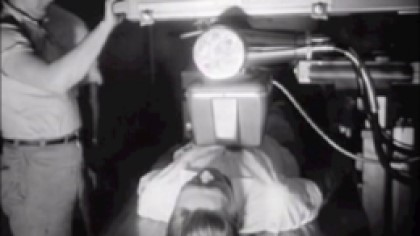
\includegraphics[width=1\linewidth]{therac.jpg}
\end{figure}

\begin{figure}
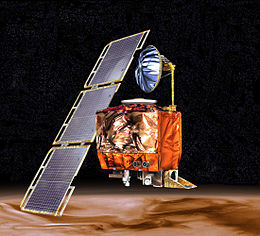
\includegraphics[width=1\linewidth]{MCO.jpg}
\end{figure}

\end{columns}
\end{frame}

\section{Verifikacija}
\begin{frame}
\frametitle{Testiranje u razvoju softvera}
\begin{columns}[c]
\column{.45\textwidth}
\begin{figure}
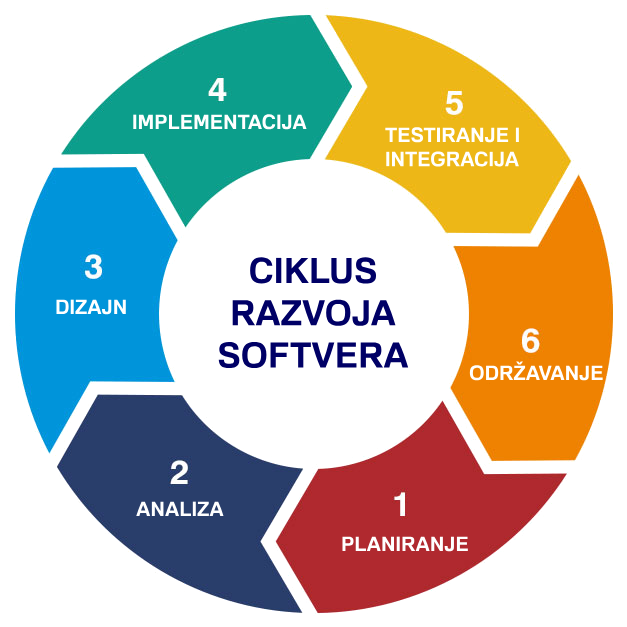
\includegraphics[width=1\linewidth]{rs.png}
\end{figure}

\column{.45\textwidth}
\epigraph{\emph{,,Program testing can be used to show the presence of bugs, but never to show their absence!‘‘}}{Edsger W. Dijkstra}

\end{columns}
\end{frame}


\begin{frame}
\frametitle{Verifikacija softvera}

\textbf{Definicija}
\begin{itemize}
\item \textit{verification = Are we building the product right?}
\item \textit{validation = Are we building the right product?}
\end{itemize}

\textbf{Podela}
\begin{enumerate}
\item Dinamička verifikacija
\begin{itemize}
\item testiranje crne kutije (funkcionalno testiranje)
\item testiranje bele kutije (strukturno testiranje)
\end{itemize}
\item Statička verifikacija
\begin{itemize}
\item simboličko izvršavanje
\item aptraktna interpretacija
\end{itemize}
\end{enumerate}
\end{frame}


\begin{frame}
\frametitle{Alati za verifikaciju softvera}

\begin{itemize}
\item \textbf{Alati za automatsko testiranje} \\
\textit{Obezbeđuju automatsko sprovođenje testova}
\begin{itemize}
\item Selenium
\item ...
\end{itemize}
\item \textbf{Formalni dokazivači ispravnosti} \\
\textit{Omogućavaju interaktivnu formulaciju matematičkog dokaza korektnosti}
\begin{itemize}
\item Isabelle/HOL
\item Coq
\item ...
\end{itemize}
\end{itemize}
\end{frame}

\section{Modeli i metrike}
\begin{frame}
\frametitle{Modeli i metrike pouzdanosti}

\begin{enumerate}
\item Deterministički modeli
\begin{itemize}
\item Holstedova metrika
\item Mek-Kejbova ciklomatična složenost
\item ...
\end{itemize}
\item Probabilistički modeli
\begin{itemize}
\item Modeli stope neuspeha
\item Modeli rasta pouzdanosti
\item ...
\end{itemize}
\end{enumerate}

\end{frame}


\begin{frame}
\frametitle{Holstedova metrika}

\begin{columns}[c]

\column{.45\textwidth}
\begin{itemize}
\item Meri se kompleksnost programa
\item Broj operatora i operanada se dovodi u vezu sa pojavom bagova
\end{itemize}

\column{.3\textwidth}
\begin{figure}
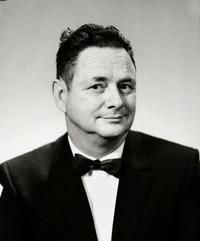
\includegraphics[width=1\linewidth]{halstead.png}
\end{figure}

\end{columns}

\end{frame}


\begin{frame}
\frametitle{Mek-Kejbova ciklomatična složenost}

\begin{columns}[c]

\column{.45\textwidth}

\begin{center}
\textbf{C = E - V + 2P} 
\end{center}

E = broj grana grafa G \\
V = broj čvorova grafa G \\
P = broj povezanih komponenti grafa G \\
G = graf kontrole toka programa 

\column{.45\textwidth}
\begin{figure}
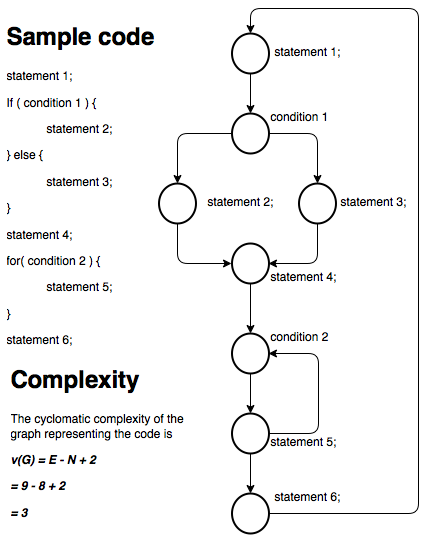
\includegraphics[width=1\linewidth]{mccabe.png}
\end{figure}

\end{columns}

\end{frame}


\begin{frame}
\frametitle{Probabilistički modeli}

\begin{itemize}

\item Greška kao verovatnosni događaj
\item Razne metode iz oblasti statistike

\end{itemize}

\textbf{Podela}
\begin{enumerate}
\item Modeli stope neuspeha
\begin{itemize}
\item prikazuju stopu otkazivanja programa po pojavi greške
\item nekoliko varijacija ovih modela
\item ...
\end{itemize}
\item Modeli rasta pouzdanosti
\begin{itemize}
\item predviđaju da li dolazi do poboljšanja pouzdanosti kroz testiranje softvera
\item dva podmodela
\item ...
\end{itemize}
\end{enumerate}

\end{frame}

\section{Budućnost}
\begin{frame}
\frametitle{Budućnost softvera}

\begin{itemize}
\item Razni alati već danas automatizuju mnoge faze razvoja
\begin{itemize}
\item Generisanje koda
\item Optimizacija
\item Debagovanje
\end{itemize}

\item Sa napretkom veštačke inteligencije i mašinskog učenja, proces razvoja može da se ubrza eksponencijalno
\item Već se radi na sistemima koji automatski generišu kod (Bayou)
\item Verujemo da će u budućnosti kod da pišu mašine, a zadatak programera će biti samo da ih kontroliše i usmerava
\end{itemize}

\end{frame}

\section{Zaključak}
\begin{frame}
\frametitle{Zaključak}
\begin{enumerate}
\item Greške su neizbežne
\item Testiranje je važno, ali ne uvek i dovoljno
\item Formalna verifikacija je ponekad neophodna
\item Mašine će zavladati svetom?
\end{enumerate}
\end{frame}

\section{Literatura}
\begin{frame}

\nocite{quinn_ethics}
\nocite{laski2009software}
\nocite{pham_reliability}
\nocite{Bayou}

\frametitle{Literatura}
\bibliographystyle{ieeetr}
\bibliography{seminarski}
\end{frame}

\begin{frame}
\frametitle{}
\begin{center}
{\Huge 01001000 01110110 01100001 01101100 01100001 00100001} \\
{\Huge (Hvala!)} \\ 
\bigskip
\bigskip
{\Huge Pitanja?}
\end{center}
\end{frame}



\end{document} 